\documentclass[a4paper]{article}

\usepackage{pdfsync}

% Use utf-8 encoding for foreign characters
\usepackage[utf8]{inputenc} 
\usepackage[english]{babel} 
% \usepackage[T1]{fontenc} 

% Setup for fullpage use
\usepackage{fullpage}

% Uncomment some of the following if you use the features
%
% Running Headers and footers
%\usepackage{fancyhdr}
% Multipart figures
%\usepackage{subfigure}
% More symbols
%\usepackage{amsmath}
%\usepackage{amssymb}
%\usepackage{latexsym}
% Surround parts of graphics with box
\usepackage{boxedminipage}

% Package for including code in the document
\usepackage{listings}

% If you want to generate a toc for each chapter (use with book)
\usepackage{minitoc}

% url package
\usepackage[hyphens]{url}

% enable clickable
\usepackage[]{hyperref}
\hypersetup{pdfborder=0 0 0}


% This is now the recommended way for checking for PDFLaTeX:
\usepackage{ifpdf}

%\newif\ifpdf
%\ifx\pdfoutput\undefined
%\pdffalse % we are not running PDFLaTeX
%\else
%\pdfoutput=1 % we are running PDFLaTeX
%\pdftrue
%\fi
\ifpdf 
\usepackage[pdftex]{graphicx} \else 
\usepackage{graphicx} \fi

% command to highlight todos
\usepackage{color}
\definecolor{Orange}{rgb}{1,0.5,0}
\newcommand{\todo}[1]{\textsf{\textbf{\textcolor{Orange}{[[#1]]}}}}

% sets the indent of the paragraph
\setlength{\parindent}{0cm}

% our commands to mark-up stuff
\newcommand{\inlinecode}[1]{\emph{#1}}
\newcommand{\toolname}[1]{\texttt{#1}}
\newcommand{\pathname}[1]{\texttt{#1}}



\title{AP GCC - CGA tool chain on unix systems} 
\author{ Torsten Becker, Frederik Rudeck, Robert Timm }

\date{2009-08-01}

\begin{document}

% sets the langauge for the listings package	
\lstset{language=C++}

\ifpdf \DeclareGraphicsExtensions{.pdf, .jpg, .tif, .png} \else \DeclareGraphicsExtensions{.eps, .jpg} \fi

\maketitle

% introduction
\begin{large}
\textbf{Introduction}\\	
\end{large}

The goal of software visualization is to give insight into complex, large-scale, existing software systems and their physical composition and relations. CGA - Call Graph Analyzer - is a software visualization infrastructure that is developed by the computer graphics systems chair of the Hasso-Plattner-Institute. The Call Graph Analyzer obtains information from various fact extraction tools and provides an interactive graph visualization system. CGA addresses the following different software engineering tasks:

\begin{itemize}
	\item Program understanding
	\item Debugging
	\item Performance analysis
	\item Quality Assurance
\end{itemize}

When CGA started, the intended operating system was Windows. The goal of this project was to port the whole CGA tool chain to Mac OS X and Linux systems. 

The growing market share of Apple computers demands for cross platform tools which are not tied to the Windows platform. With our implementation, we provide an alternative fact extraction tool chain based on common unix development tools like GCC and GDB. This enables CGA to be used to instrument a wider range of projects, because now it is possible to analyse systems which only support the GCC compiler. 
\newpage

\tableofcontents
\newpage


% \addtolength{\parskip}{\baselineskip}
\setlength{\parskip}{0.27cm}


%!TEX root = ../ap_gcc.tex

\section{Results}

This section provides a short overview on what we achieved during the project.

\subsection{CMake build enviroment} We switched the build environment of CGA from Visual Studio to CMake. This enables the same build configuration to manage the build process on several platforms for several compilers by generating makefiles or project files  for the most common IDEs.

We tested this system for Visual C++ on Windows and for Makefiles on Linux and Mac OS X. It is very likely that this will also work without any tweaks for KDevelop, Xcode and many many more.

\subsection{Callmon runtime library} We implemented a callmon runtime library for applications and libraries build with GCC. This library features a lock free path from call event to log file (even in multithreaded environments using atomic operations), starting and stopping of the logging process using file system event APIs and asynchronous I/O to handle writing of log files as efficient as possible. Finally we benchmarked I/O throughput of up to 70MB per second (MacBook Pro Unibody running ioQuake3).

\subsection{Patch and Patchclean} We implemented tools to patch executables and libraries on Linux and Mac OS X. These tools store patch information in a very efficient way to binary patch files, which consume very little disk space.

\todo{little disk space?}

\subsection{Metacreator} To port metacreator to Linux and Mac OS X we just implemented the DiaInterface. So we were able to port the whole tool with very little code changes.

We added a class which gets instantiated from the DiaFactory and then interfaces with GDB to obtain debugging information like file names, line numbers of functions and call sites. Caching allows to reduce the communication with GDB to a minimum.

\subsection{Cross platform fixes for the CGA application and toolbar}

Finally we fixed several issues in the CGA application to allow the operation on Windows and Unix platforms.

Besides some fixes for cross platform compatibility, the CGA Toolbar is exactly the same and can be used as usual for starting and stopping the logging process.

\todo{genauer}
 

\newpage

\section{Challenges} This section describes challenges we had to face while porting the CGA framework to Mac OS X and Linux.

\subsection{Complexity} The first challenge was the complexity of CGA. The main application itself contains more than 70.000 lines of code. The whole distribution consists of about 170.000 lines of code. 

Furthermore, analyzing an application using CGA requires several distinct steps, like adjusting the build process of the application that is getting analyzed, patching the applications binary and post processing the data collected while running the application. Porting this tool chain to another operating system requieres a deep understanding of all those processes on one hand, and on the other hand a good idea how to realize all those details on the target platform.

\subsection{Platform specifics} The whole CGA tool chain relies on lots of platform specific mechanisms like binary patching and collecting of information from the dynamic linker. A big challenge was to find ways to get all the information needed on both target platforms. 

Parts of our implementation rely on GCC and GDB, which are both available on Linux and Mac OS X. They provided us with a good point of abstraction to hide platform specific details. But even with those tools, certain thing behave differently on both platforms. Writing into a binary with GDB does not work on Mac OS X, but does work on Linux. Function call addresses reported by the GCC instrument function mechanism may be wrong on Linux. Just to name two examples. 

TODO DLLMAIN

\subsection{Compiler specifics} The main instrumentation mechanism if based on a feature provided by the compiler. The Microsoft Visual C++ can insert calls to instrumentation functions right after a function was called and right before a function returns. The mechanism in general is the same using GCC, but the differences appear when it comes to details. 

On Visual C++, it is possible to compile a function \emph{naked}, which removes functions prolog and epilog and lets the programmer implement them himself. This feature enables the function to have a certain view on the stack, because the implementation itself is responsable for creating the stack frame, adjusting stack pointers and so on. So as a \emph{naked} function starts, it has the same view on the stack as the function which called it. This is great for the implementation of the instrumentation functions. GCC as well does provide this feature, but, it is not supported on x86 platforms. So we had to work around this situation.

Some data types, like hash\_map, which are not part of the C++ Standard, have different names and reside in different namespaces on different compilers.

\subsection{IDE specifics} While introducing the CMake based build system in CGA, we found ourselves in front of a complex and highly platform specific Visual Studio solution with lots of inter project dependencies. It contained lots of custom build steps, like Qt preprocessing steps (uic and moc) and post build steps to get, for example, unit testing data in place.

Furthermore the solution was a grown structure, so several obsolete code files still exist in the source tree, but are excluded from the build process. Includes defined using the Visual Studio project were missing in the source files which actually needed them. Just to name a few pitfalls.

\subsection{Backport to Windows}

\subsection{Mergen}

\subsection{Qt did a great job} In general, we have to say, that Qt did a great job. Without the platform independence of not only all the GUI code, it would not have been possible to port CGA in such a short time periode. 
 

\newpage

\section{Requirements} This section describes some version requirements for the tools we are using. 

\subsection{Summary}
\begin{itemize}
  \item A patched version of VRS (see below for details)
	\item GCC tested on 4.2, 4.3 (need minimum version 4.2)
	\item GDB tested on 6.3, 6.8
	\item BINUTILS tested on 2.19.1, XCode 3.1.3
\end{itemize}

\subsection{Patched version of VRS} In order to get CGA running on Mac OS X and Linux, we needed to apply three patches to VRS. One of them is necessary to get VRS to compile, the second one is a header only fix for VRS, without it, CGA would not compile and the third one is a workaround for a crash in VRS, happening when using CGA. The three patches can be downloaded at GitHub:

\begin{itemize}
\item http://github.com/torsten/ap\_gcc/blob/b4847070f55198fcee57102c959adc0c4c794b5c/vrs-trunk-r6691-gcc-build-fix.patch
\item http://github.com/torsten/ap\_gcc/blob/b4847070f55198fcee57102c959adc0c4c794b5c/vrs-trunk-r6691-linux-cga-context-foo-crash-workaround.patch
\item http://github.com/torsten/ap\_gcc/blob/b4847070f55198fcee57102c959adc0c4c794b5c/vrs-trunk-r6691-mac-qt4-debug-only.patch
\end{itemize}

Please note, that all the three patches are made for VRS trunk revision 6691.

\subsection{GCC Version} We need a GCC version, which is greater than or equal to version 4.2 because we are using some functionality which appeared in GCC version 4.2 for the first time.\\

For example with the function \emph{\_\_sync\_bool\_compare\_and\_swap} GCC provides us with a cross platform way to test and set a variable in an atomic way. This is used several times in the lock free callmon implementation and is therefor essential.\\

We as well tested our code on GCC 4.3 without any problems.

\subsection{GDB Version} Our implementation of the metacreator was tested on GDB version 6.3 (on Apple Mac OS X) and 6.8 (on Ubuntu Debian Linux).\\

We do not depend on any functionality which was introduced in version 6.3, so our implementation may also run on older and/or newer versions of GDB. But since we are using GDB in a terminal way (writing commands to it and reading its output), we highly depend on the formatting of GDBs output. Even between version 6.3 and 6.8 there were several small differences like additional line breaks in GDBs output.\\

But extending our implementation to handle more versions of GDB is as easy as fixing the regular expressions parsing the GDB output.

\subsection{Binutils} On Linux we are using \emph{objdump} and \emph{nm} from the binutils distribution. All our code was tested with version 2.19.1 of these tools. On Mac OS X we a using \emph{otool} and \emph{nm} as provided by Apple bundled with XCode version 3.1.3.\\

Like in the GDB case we are parsing the output using regular expressions, so changes in the output format of these tools are likely to break our parsing, but again, only some regular expression need to be adjusted.
 

\newpage

\section{CMake Build System}
keine special coding richtlinien

\subsection{Qt specific build steps}
wo landen die uic generierten dateien

\subsection{on Windows}

\todo{CMake GUI - grouped view}

\subsection{on Linux}

\subsection{on Mac OS X} 
 

\newpage

%!TEX root = ../ap_gcc.tex

\section{Unix fact extraction mechanism in detail}

In this section we want to explain the unix fact extraction mechanism in more detail. Especially we want to explain how we implemented the callmon library, the executable patching mechanism and metacreator.

\subsection{Overview}

First of all we want to give a quick overview about the whole workflow of the fact extraction tool chain. These are the steps if you want to instrument your application and visualize the trace in CGA:

\begin{enumerate}
	\item Building the application with special compiler flags and linking the callmon.{dll,dylib,so}.
	\item Patching the executable results in an executable with just NOPs and a patch file (patch clean).
	\item Patching the executable with the help of an include/exclude file so that we just have specific logging enabled (patch).
	\item Executing the application.
	\item Start logging with the cga toolbar creates a pre modinfo file.
	\item During the logging callmon writes cmlog files for every thread.
	\item Stop logging with the cga toolbar creates a post modinfo file.
	\item The metacreator takes the cmlog and modinfo files and creates a .callmon file
	\item Import and visualize the trace with CGA.
\end{enumerate}

The unix fact extraction mechanism is a non-intrusive, light-weight way for logging function calls in C/C++ software systems that are built with GCC version 4.2 or higher. Callmon is used to log the sequence of function calls from a running application. Time stamps are obtained for both entry and exit points of each function. The logging mechanism does not slow down the users application when being deactivated. This is obtained by patching the executable and libraries files of the application. All assembler instructions, which are needed for logging are replaced by assembler NOPs. If the user wants to log certain activities he can patch the executable again so that the logging for this functions are now active. For more detailed information about the process have a look at the tutorial section \ref{sec:Tutorial}.

\subsection{Callmon}

The central element of the tracing mechanism is callmon. Callmon is a static library, which you have to link against the application you want to instrument. But the most important part is the GCC parameter \inlinecode{-finstrument-functions}. We will explain this later in more detail. To get an overview about the classes which are involved in the tracing mechanism have a look at figure \ref{fig:unixfe_figure1}.

\begin{figure}[ht]
\centering
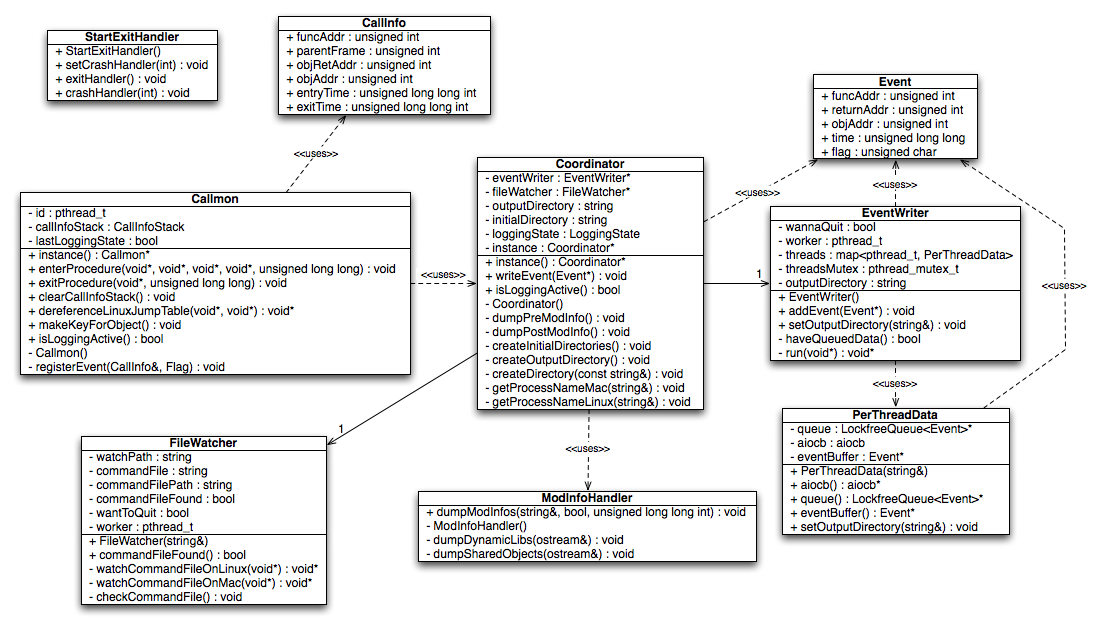
\includegraphics[width=18cm]{images/callmon_class_diagram}
\caption{Class diagram of the callmon library}\label{fig:unixfe_figure1}
\end{figure}

The \verb=StartExitHandler= \todo{new font here? use it all over?} helps to set up crash handlers for the most common signals (SIGINT, SIGILL, SIGSEGV, SIGFPE, SIGTERM, SIGABRT, SIGBUS, SIGHUP)\footnote{\url{http://en.wikipedia.org/wiki/Signal_(computing)}} and an exit handler right after startup (before main). We ensure that the constructor of the \verb=StartExitHandler= is executed before the main routine of the application with the help of a static variable. Static variables are initialized before the first call of the applications main routine. The \verb=exithandler()= function deletes the \verb=Coordinator= instance. If the application crashes the crash handler gets executed, which processes just a normal shutdown and cleanup.

\verb=Callmon= provides the functionality to log function enters and exists. Every thread of the application has its own \verb=Callmon= object. The \verb=Coordinator= is responsible to create the \verb=EventWriter=, the \verb=FileWatcher= and the directory structure for the log files. It also coordinates if callmon is allowed to log an event. The \verb=EventWriter= runs in its own thread and receives events from all the applications threads through a lock free queue. It uses asynchronous I/O to fill the thread specific log files. The \verb=FileWatcher= runs also in its own thread and listens on events of the file system. If a file called callmond.cmd is created or deleted we indicate this with a boolean. The \verb=ModInfoHandler= is responsible to write at the beginning and the end of the logging a list of used libraries and their start address to a modinfo file. Some classes are explained in more detail in the next sections.

As mentioned more early, one of the key elements is the GCC parameter -finstrument-functions. With this option GCC inserts calls to \verb= __cyg_profile_func_enter()= and \verb=__cyg_profile_func_exit()=. When an instrumented function is called, \verb= __cyg_profile_func_enter()= is also called, passing in the address of the function called as \verb=funcAddress= and the address from which the function was called as \verb=callSite=. When a function exits, the \verb=__cyg_profile_func_exit()= function is called, passing the function's address as \verb=funcAddress= and the actual site from which the function exits as \verb=callSite=.

We implemented both functions (see callmon.cpp), which collect the following data if logging is active:
\begin{itemize}
	\item Function address
	\item Call site
	\item Frame pointer
	\item Parent frame pointer
	\item Object pointer (this pointer)
	\item Entry and exit time
\end{itemize}

On Linux when a function of a shared library gets called from the main executable, \verb=__cyg_profile_func_enter()= reports the wrong function address. It just tells the address in the jump table, not where the real function code is located. Therefore we have to correct the function address with the help of \verb=dereferenceLinuxJumpTable()=, which searches the jump table and finds the real address.

\begin{figure}[ht]
\centering
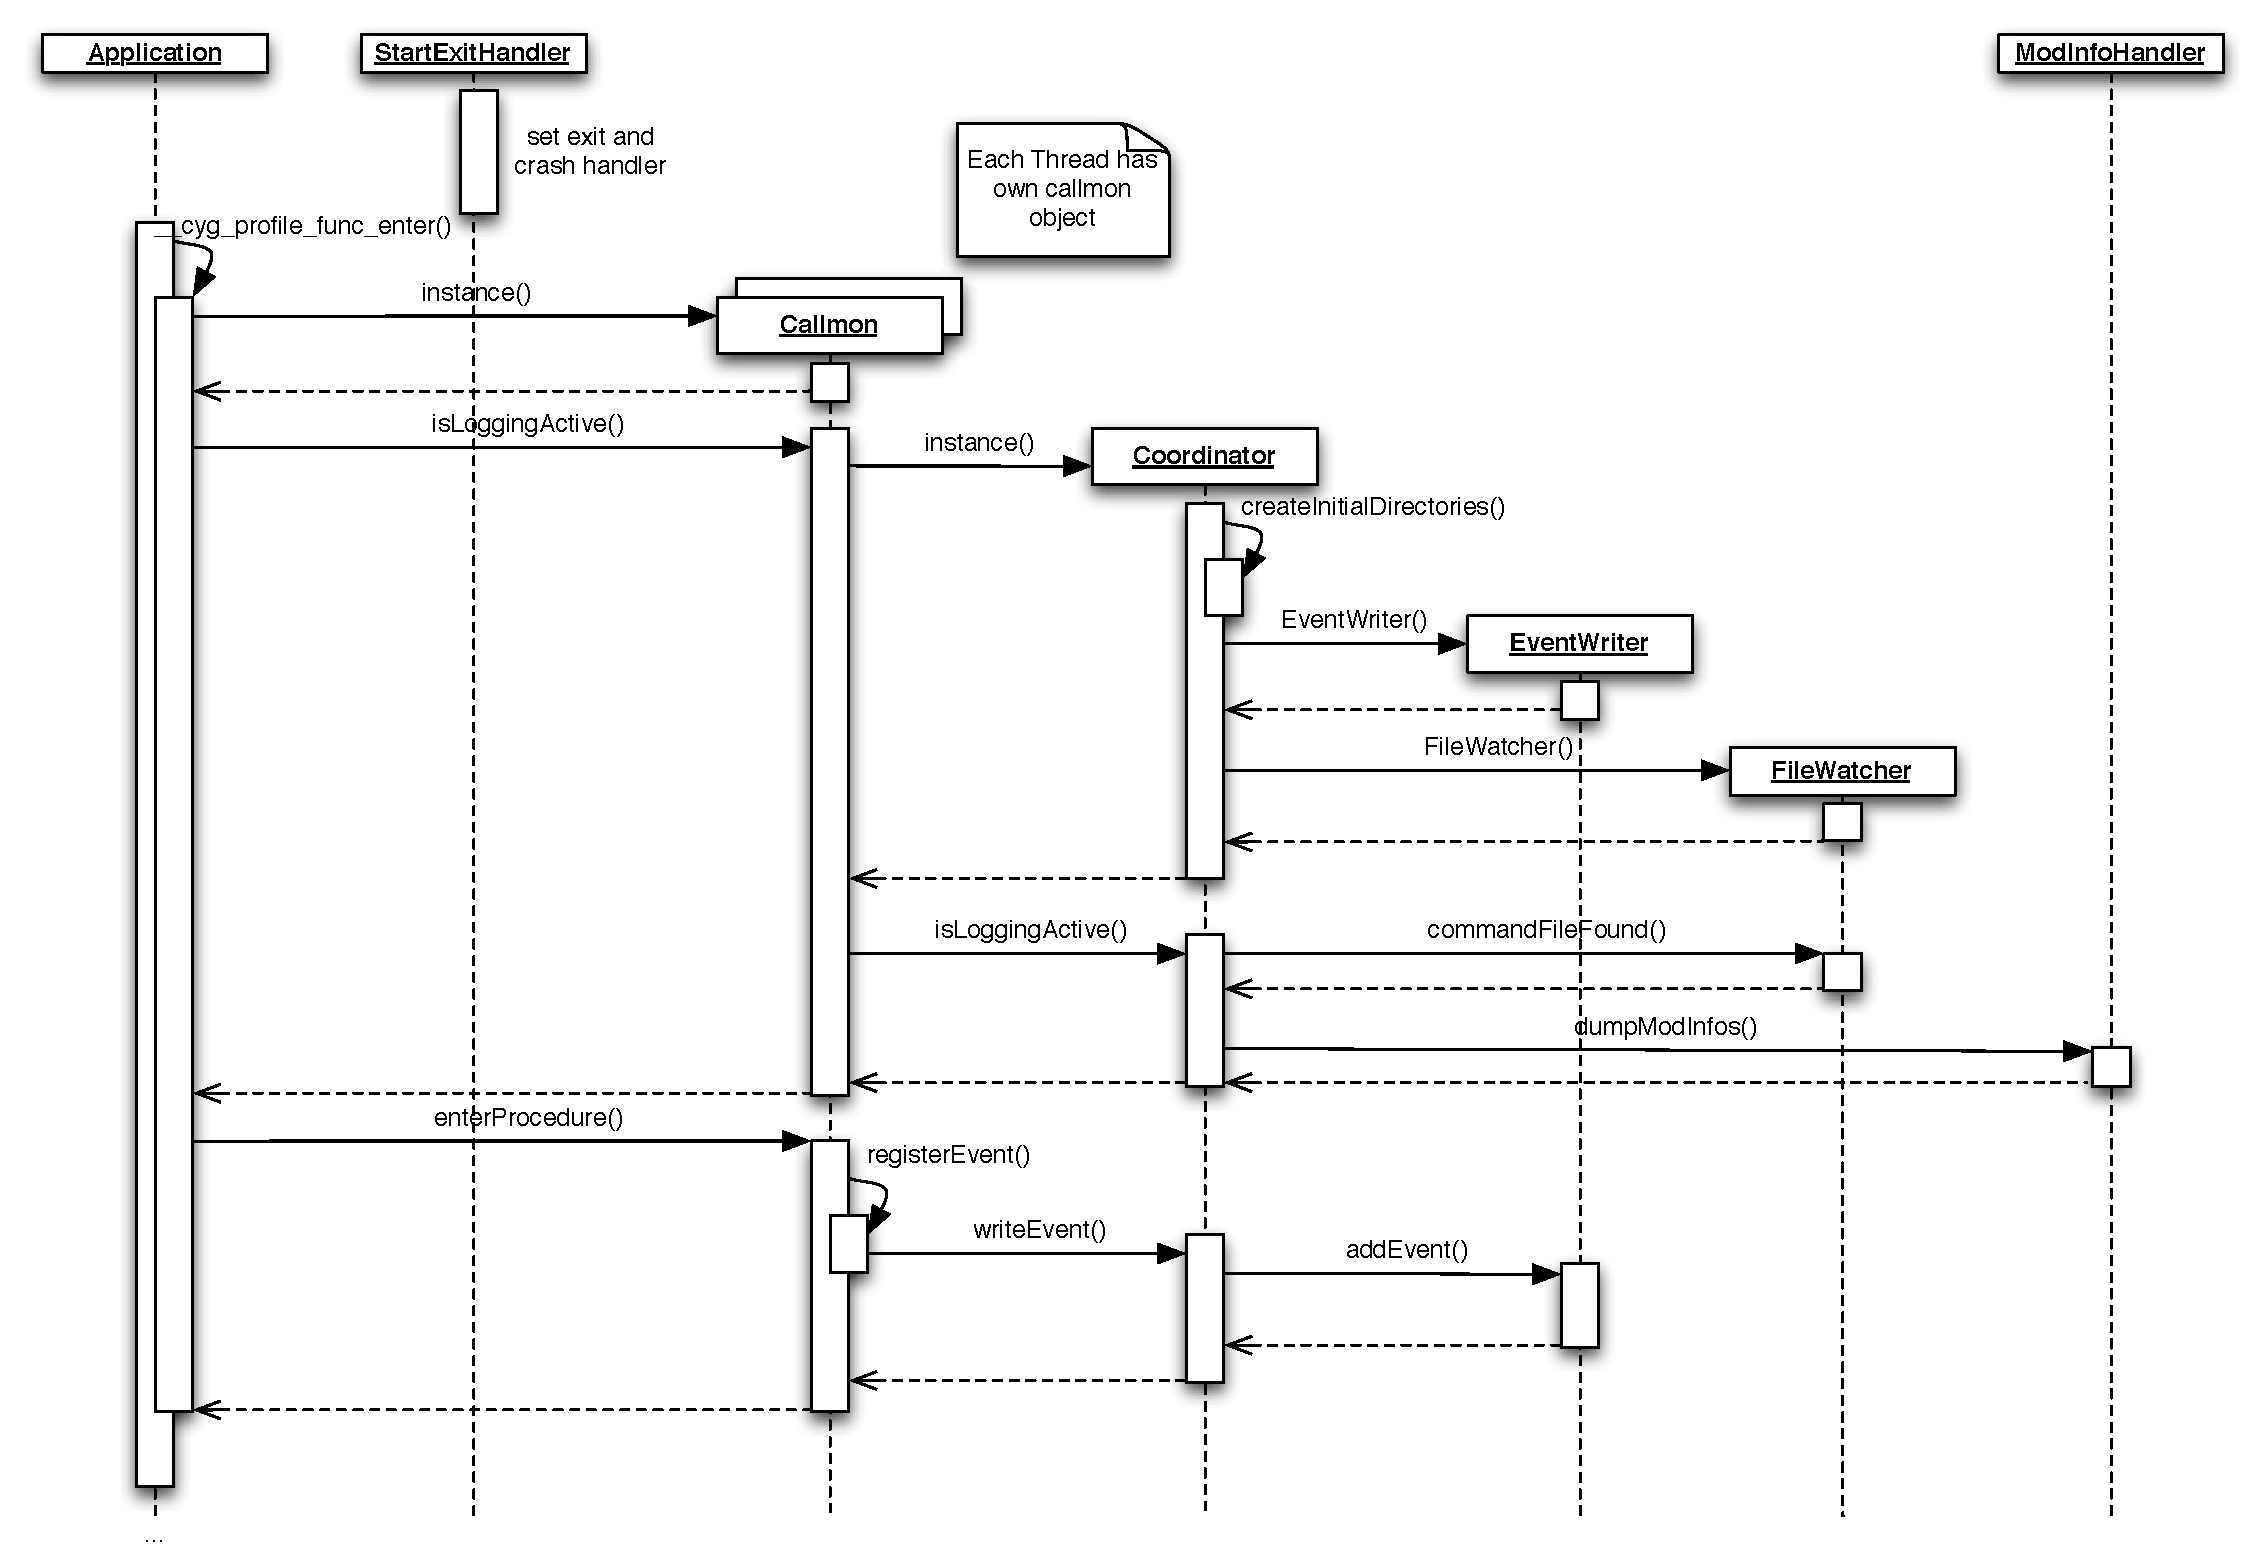
\includegraphics[width=18cm]{images/callmon_sequence_diagram}
\caption{Sequence diagram of the function enter process}\label{fig:unixfe_figure2}
\end{figure}

Figure \ref{fig:unixfe_figure2} illustrates a simplified event logging process for the first \verb=__cyg_profile_func_enter()= in which we assume that logging is enabled. If the user starts the application the constructor of the \verb=StartExitHandler= is executed up front and the exit and crash handler is set up. In the next step the \verb=__cyg_profile_func_enter()= is called. On Mac OS X and Linux exists no DllMain mechanism, so we have to use lazy initialization and thread-local storage to address this problem. A callmon instance is requested and created on demand if there is no instance for this thread. The pointer to the callmon instance is stored in the thread-local storage. After the lazy	initialization of the callmon object we check if logging is active. To determine if we are allowed to log an event, we need to create a coordinator (singleton), which is also responsible to initialize the event writer and file watcher (detailed information can be found in the following sections). Both the event writer and file watcher run in their own thread. After this, callmon can ask the coordinator if logging is active or not. The whole logging mechanism is enabled if the file watcher finds a \verb=callom.cmd= file in the callmon home directory. If this was the start of a new logging procedure we also write a pre modinfo file to the specified output directory.

In the next step \verb=__cyg_profile_func_enter()= collects the whole data we need to write an event to the thread specific log file. This data is passed to the \verb=enterProcedure()= of the callmon instance. In this function we push a new \verb=CallInfo= object on our shadow stack. On the one hand we need the shadow stack to recognize if there was an exception during the execution, because then we will have a different return behavior of the function. On the other hand the shadow stack is needed to address the problem if we have an unprofiled function call between two profiled functions. Then we call the \verb=registerEvent()= function, which creates a new \verb=Event= object. The Event is then written with the help of the \verb=EventWriter= to a log file.

The whole procedure for \verb=__cyg_profile_func_exit()= is very similar, beside that the \verb=exitProcedure()= pops the shadow stack until we find a call record that matches the current stack layout. If we did not find a call record that matches we register an exceptional event.

The structure of the event which is also written to the cmlog files looks like the following:
\begin{itemize}
	\item Function address
	\item Return address
	\item Object address
	\item Entry or exit time
	\item Flag (entry, exit or exception)
\end{itemize}

\subsubsection{Coordinator}

The \verb=Coordinator= class uses the singleton design pattern so that we just have one \verb=Coordinator= instance at a time. One of the important tasks of the class is to set up the initial directory structure where callmon stores the log and mod info files. Therefore the function \verb=createInitialDirectories()= is called in the constructor, which creates the following directory structure:

\begin{verbatim}
  CALLMON_HOME|./logs/<appname>/
\end{verbatim}

On Mac OS X the name of the currently running application ($<$appname$>$) is determined with the help of the \verb=kinfo_proc= structure. On linux we use the process file system, which is a pseudo file system used to access process information from the kernel. We get the name of the application by resolving 

\begin{verbatim}
  /proc/<pid>/exe (symbolic link)	
\end{verbatim}

Another important task of the \verb=Coordinator= is to create the \verb=EventWriter= and \verb=FileWatcher=, which will be explained later in more detail. But the most important functionality of the \verb=Coordinator= is to indicate if callmon is allowed to log the function enters and exits in a lockfree way, even in multithreaded environments. This is accomplished by using atomic operations. Since version 4.2 GCC provides a function called \verb=__sync_bool_compare_and_swap()=, which sets and test a variable in an atomic way. The \verb=Coordinator= instance asks the \verb=FileWatcher= if logging is active or not. If logging is active we have to check if we are at the beginning of a new logging cycle. At the beginning of a logging cycle we have to set up certain things such as creating the output directory for the log files, write a pre modinfo file and set the output directory of the \verb=FileWatcher=. The output directory for the current trace is:

\begin{verbatim}
  CALLMON_HOME|./logs/<appname>/<date_time>
\end{verbatim}

If we are not allowed to log we have to check if we are at the end of a logging cycle. At the end of a logging cycle we write a post modinfo file to the current output directory.

\subsubsection{Modinfo handler}

The \verb=ModInfoHandler= provides the functionality to write a pre modinfo file at the beginning of a new trace and a post modinfo file at the end of the trace. The first line of the modinfo file is the \verb=queryPerformanceFrequency=, which is not used anymore. To be consistent with the Windows callmon implementation we still write this as the first line in the modinfo file. The central element of the modinfo file is the list of libraries and their start addresses the application is using. The format of the file looks like this:

\begin{verbatim}
  queryPerformanceFrequency: 1
  00000000 /path/to/lib
  ...
\end{verbatim}

To get the start address and the path of the libraries on Mac OS X we use the following functions the linker provides. The function \verb=_dyld_image_count()= returns the current number of images mapped in by the dynamic linker. The start address can be resolved with the help of \verb=_dyld_get_image_vmaddr_slide(image_index)= and to get the name of the library we use \verb=_dyld_get_image_name(image_index)=, which returns the name of the image.

On Linux the \verb=dl_iterate_phdr()= function walks through the list of an application's shared objects and calls the function callback once for each object. The first of the three parameters the callback gets, is a pointer to a \verb=dl_phdr_info= structure, which contains the start address and the name of the shared object.

\todo{TODO: explain for what modinfo files are useful}

\subsubsection{Filesystem events}

The \verb=CGA Toolbar= is a simple QT application which simplifies the whole logging process. Besides some small fixes for cross platform compatibility it is exactly the same application as the previous Windows version. With the toolbar the user can start and stop the logging mechanism and start the metacreator for traces of a specific application. The interesting part of the toolbar is in order to start and stop the logging mechanism, it creates an empty file called \verb=callmon.cmd= at the path specified by the \verb=CALLMON_HOME= environment variable. To stop logging the toolbar removes the \verb=callmon.cmd= file.

That is the reason why we need to listen on filesystem events to start and stop logging. In both cases we listen for changes on a specific path and set a variable to true if we find the \verb=callmon.cmd= file or to false if not.

On Mac OS X we use the kernel event notification mechanism \verb=kqueue= and \verb=kevent=. The \verb=kqueue()= system call provides a generic method of notifying the user when an kernel event happens or a condition holds, based on the results of small pieces of kernel code termed filters. The \verb=kevent()= system call is used to register events with the queue, and return any pending events to the user. The only downside of this solution is that we do not get the exact change as an event, we just get the event that a file was created or deleted at the specified path. So we have to check manually with \verb=open(file)= if the file exists. The \verb=kevent()= system call is blocking for a specified timeout or until there is a pending event. In our case we specified a timeout of one second, so that we can interrupt the loop if we want to suspend the \verb=FileWatcher= thread.

The Linux way uses \verb=inotify= which is a Linux kernel subsystem that provides file system event notification. The \verb=inotify_init()= call creates a new instance and returns a file descriptor which all events are read from. With the help of \verb=inotify_add_watch()= we add a new watch for the specified path. We can now call \verb=read= on the file descriptor. This call will block until we get an event. The \verb=inotify_event= structure provides us with enough information so that we can check if the \verb=callmon.cmd= file was created or deleted.

\subsubsection{Event writer} 

event writer (own thread), PerThreadData, setOutputdirectory, Mutex

The lockfree queue is thread safe as long as there is only one reader and one writer. It has a static size which has to be provided at initialization. \todo{TODO: explain in more detail}

\subsubsection{Asynchronous I/O}

We use asynchronous I/O to write the logged function entries and exits to a thread specific log file. The \verb=EventWriter= runs in its own thread and stores the received events, as described in the previous section, in a lockfree queue. If the \verb=EventWriter= thread is scheduled we check if there are any events in the queue and write them to the log file. A very simple approach to write the events to the log file would be synchronous I/O, which blocks the progress of a program until the operations are completed. The alternative is to start the communication and then perform processing that does not require that the I/O has completed. This is called asynchronous I/O and is much more efficient then synchronous I/O.

To perform asynchronous I/O we use the POSIX standard for asynchronous input and output. \verb=aio_write()= gets as parameter a \verb=aiocb= structure which stores a file descriptor, file offset, the location of the buffer we want to write and the length of transfer. For more specific information have a look at the \verb=aio= man page.

\subsection{Patch and Patchclean}

Unfortunately the original patch and patchclean tools had some implementation specific limitations which made a direct port to UNIX hardly feasible.

\todo{Reasons: Windows API, PE code, DIA API, nur enter}

Also the requirements on Linux and Mac OS X where different because of the fact that GCC always compiles the exit instrumentation into the functions and enforces its call on all ways out of a function.

Because of the above mentioned reasons we decided to re-implement the patching tool chain for Linux and Mac OS X.  This 2 new UNIX patching tools reside in the \emph{factextraction/unix/unixfactextraction/} directory.

\todo{Explain architecture, similar to windows, patch files (qdatastream), }


\subsubsection{ELF patching} 

file specifics, offsets, objdump, see requirements


\subsubsection{Mach-O patching}




\subsection{Metacreator} 

\subsubsection{Line number caching} 
 

\newpage

%!TEX root = ../ap_gcc.tex

\section{Tutorial}
\label{sec:Tutorial}

This section shows how to profile a project step by step. In general, the process is quite similar to the process needed to profile a project with the Windows version of callmon. Big differences only appear in the build configuration due to differences in the compiler switches needed by GCC.

\subsection{Preparing the build process} How to prepare the build process.

\subsubsection{Parameters to GCC} This is a list of parameters needed by GCC when profiling with unix fact extraction.

\paragraph{Compile with -g} Enable debug information.

With this option enabled, GCC builds debug information into the resulting binary. This is needed by metacreator to resolve source file name, line numbers and other valuable debugging information.

Note that you can still compile with optimizations enabled (\inlinecode{-O2} and friends) since our mechanism finds multiple enters and exists per function.

\paragraph{Compile with -finstrument-functions} Enable instrumentation.

This GCC parameter is the key. With this option enabled, GCC inserts calls to instrumentation functions right after a function was called and right before a function returns. If you do not provide this option in the compilation process, no calls will be made to the unix callmon library, and therefor no profiling information can be retrieved.

\paragraph{Compile with -fno-inline} Disable inlining of functions.

This disables the inlining of functions which is done explicitly by the developer or automatically by the compiler to optimize execution speed by eliminating function call overhead.

Since we are profiling on a function execution level, we cannot profile inlined function, so all the functions inlined by the compiler cannot appear in the call graph. To be sure this cannot happen, use \inlinecode{-fno-inline} as a GCC option. You might skip this if you want. You still might get good profiling results for the calls you are interested in, but you have been warned!

\paragraph{Link unixcallmon library as the last library} Ensure the right profiling functions are used.

It might happen, that other libraries as well provide the profiling functions that unix callmon lib provides (glib is an example for that). If this happens, it is important to ensure that the versions of the unix callmon lib are the ones linked in. This is done by adding the \inlinecode{-lunixcallmon\_lib} parameter as the last one.

\paragraph{On Linux, link with -Wl,-Bsymbolic} Make function calls patchable.

\todo{explain this case more in detail, just happens with .so s, etc.}

Without this option, symbolic function call information is removed from the resulting binary on Linux. This prevents \toolname{cga\_patch} and \toolname{cga\_patchclean} from finding the call locations and makes it impossible to remove those calls from the binary. 

\paragraph{Build with absolute path to source} Ensure CGA can find source files.

To ensure that CGA can find the source files for the source code viewer, you need to provide GCC with the absolute path to the source file while compiling.

\subsubsection{Putting it all together}

If the project you want to analyze is build using make, you might want to add the following to the projects Makefile:

\begin{verbatim}
  CFLAG   += -g -finstrument-functions -fno-inline 
  LDFLAGS += -Wl,-Bsymbolic -L/path/to/callmonlib -lunixcallmon_lib
\end{verbatim}

\subsection{Building the application}

With all the above mentioned set up, you build your project as usual, e.g. by typing \toolname{make}.

To enable the following command lines to work you might have to move the executables \toolname{cga\_patchclean} and \toolname{cga\_patch} to some location in your \inlinecode{PATH} for symlink them accordingly.

\subsection{Patching the executable}

As soon as the build process has finished, you end up with an executable or library which has all the profiling mechanisms build in. At this point, every single function which was just compiled by GCC is now enriched by profiling logic. Since this may be a lot, you might want to exclude several functions or groups of functions from the profiling process. This is done by patching the binary. Technically, the calls to the instrumentation functions get overwritten by NOP operations, so almost no overhead is involved in calling functions removed from the profiling process.

\subsubsection{Patch clean} The first thing to do is call \toolname{cga\_patchclean} on the binary like this:
\begin{verbatim}
  $ cga_patchclean myBinary myBinary.patch
\end{verbatim}
The first parameter specifies the binary to patch. The second parameter specifies a patch file name. In this patch file, \toolname{cga\_patchclean} will write out all the locations from which profiling calls were removed along with the opcodes removed that realized the call. This information is needed by \toolname{cga\_patch} to re-include the call opcodes for certain functions in the next step.

\subsubsection{Patch} At this point, profiling logic is re-added to the functions of interest. This is done by specifying two groups of function name patterns in a pattern file. This is exactly the same like for Windows callmon.

Provide a list of patterns in the include section, as well a list of patterns in the exclude section. Then, call patch like this:

\begin{verbatim}
  $ cga_patch myBinary myBinary.patch myPatternsFile.txt
\end{verbatim}

You may leave the patterns file parameter empty to re-include all functions in the profiling process. Like this:

\begin{verbatim}
  $ cga_patch myBinary myBinary.patch
\end{verbatim}

\subsection{Using CGA Toolbar}

The CGA Toolbar can be used as usual. It needs to set up the environment variable \inlinecode{CALLMON\_HOME}. This variable has to contain the path, where the log files are created. So lets say, you have a directory structure like this:

\begin{verbatim}
  <working directory>/
  |
  |- myBinary
  |- myBinary.patch
  |- myPatternsFile.txt
\end{verbatim}

Create a directory where the CGA Toolbar can operate on, like this:

\begin{verbatim}
  $ mkdir -p logs/myBinary
\end{verbatim}

You end up with a directory structure like this:

\begin{verbatim}
  <working directory>/
  |
  |- logs/
  |  |
  |  |- myBinary/
  |     |
  |     |
  |
  |- myBinary
  |- myBinary.patch
  |- myPatternsFile.txt
\end{verbatim}

Now, fire up the CGA Toolbar like this:

\begin{verbatim}
  $ CALLMON_HOME="<working directory>" cgatoolbar
\end{verbatim}

The string \emph{myBinary} should now show up in the drop down menu in the CGA Toolbar. If you now hit the start button, CGA Toolbar will create a file called \pathname{callmon.cmd}:

\begin{verbatim}
  <working directory>/
  |
  |- logs/
  |  |
  |  |- myBinary/
  |     |
  |     |- callmon.cmd
  |
  |- myBinary
  |- myBinary.patch
  |- myPatternsFile.txt
\end{verbatim}

This tells callmon to log function calls. Hitting the stop button will remove this file. You are now ready to run your application and record profiling information.

\subsection{Running the application}

Run the application as usual for example like this:

\begin{verbatim}
  $ ./myBinary -someParameter=someValue
\end{verbatim}

If you now press start and stop on the CGA Toolbar, new traces will be generated. Each trace will reside in the \pathname{logs/myBinary/} directory. Each trace will be put into its own directory depending on the date and time the logging started at. So after you created several traces, you might end up with a directory structure like this:   

\begin{verbatim}
  <working directory>/
  |
  |- logs/
  |  |
  |  |- myBinary/
  |     |
  |     |- callmon.cmd
  |     |- 090229_143523
  |     |- 090229_143542
  |     |- 090229_143559
  |     |- 090229_143614
  |
  |- myBinary
  |- myBinary.patch
  |- myPatternsFile.txt
\end{verbatim}

Each trace directory now contains .cmlog files, each of them representing the events that occured in one thread and .modinfo files, that contain the dynamic library state when logging started and as well when logging ended. So the directory for one trace may look like this: 

\begin{verbatim}
  090229_143542/
  |
  |-profile_4243_b8bfa41d.cmlog
  |-profile_4243_b8bfd411.cmlog
  |-profile_4243_b1ad00d2.cmlog
  |-profile_4243_pre.modinfo
  |-profile_4243_post.modinfo
\end{verbatim}

The first number in the .cmlog filename describes the process identifier, the second number in hexadecimal describes the thread identifier. The .modinfo filenames as well contain the process identifier.

\subsection{Using Metacreator}

The next step is to enrich the collected information by running metacreator. Therefor you simple fire up metacreator and provide it with a traces directory as parameter, like this:

\begin{verbatim}
  $ metacreator ./logs/myBinary/090229_143542
\end{verbatim}

Depending on the amount of events you collected, metacreator will take some time now. For all the logged calls, metacreator will now resolve debugging information from the binary. Once finished, a new .callmon file was created in the traces directory. So it should look like this now:

\begin{verbatim}
  090229_143542/
  |
  |-profile_4243_b8bfa41d.cmlog
  |-profile_4243_b8bfd411.cmlog
  |-profile_4243_b1ad00d2.cmlog
  |-profile_4243_pre.modinfo
  |-profile_4243_post.modinfo
  |-profile_4243.callmon
\end{verbatim}

All the preparations are done now. You can now start up CGA and load the trace.

\subsection{Loading the trace(s) into CGA} Start the CGA executable, create a new project. Then, select manage traces, click the add button, select your .callmon file and let CGA import the trace.
 

\newpage

\section{Guideline - Code that builds on GCC and Visual C++}
This section contains a list of the most common problems we found in the code of CGA and their solution.

\subsection{Paths} To be valid on Windows and Unix platforms, a path \textbf{must not} contain backslashes as separators. The only valid path separator for both platforms is the slash symbol \textbf{/}. So a valid path looks like this: 
\begin{verbatim}
	"this/is/a/valid/path" 
\end{verbatim}

\subsection{Const correctness} 

\subsection{Templates} The GCC's parser for template type name behaves slightly different than the Visual C++ ones. For example this is a valid definition in Visual C++: 
\begin{verbatim}
	std::list<std::pair<int, int>> myListOfIntPairs; 
\end{verbatim}

This is \textbf{not} valid while compiling with GCC. You have to separate \textbf{>} symbols using a space, else, GCC will throw a parser error. So this is the valid equivalent, which compiles on GCC and Visual C++: 
\begin{verbatim}
	std::list<std::pair<int, int> > myListOfIntPairs; 
\end{verbatim}

\subsection{Member function declarations} When declaring a member function inside the class statement, some people tent to prepend the name of the class to the method name. This may increase readability when inheriting several levels:
\begin{verbatim}
    class A {
    public:
        virtual void A::funcFromA();
    };
    
    class B : public A {
    public:
        virtual void A::funcFromA();
        virtual void B::funcFromB();
    };
    
    class C : public B {
    public:
        virtual void A::funcFromA();
        virtual void B::funcFromB();
        virtual void C::funcFromC();
    };
\end{verbatim}

The problem is, this \textbf{is not} a valid syntax for GCC. You \textbf{must not} prepend the class name to the member function. So the above declaration is valid for GCC like this:
\begin{verbatim}
    class A {
    public:
        virtual void funcFromA();
    };
    
    class B : public A {
    public:
        virtual void funcFromA();
        virtual void funcFromB();
    };
    
    class C : public B {
    public:
        virtual void funcFromA();
        virtual void funcFromB();
        virtual void funcFromC();
    };
\end{verbatim}

\subsection{windows.h} You \textbf{must not} include windows.h because all the types and functions provided by windows.h are highly Windows specific and will not compile nor run on other platforms. In general you will find the same functionality in QtCore. When using QtCore's functionality, it is easy to compile and run the code on all the platforms supported by Qt.

\subsection{for each() vs. foreach() vs. for()} Visual C++ provides a construct which looks like this:
\begin{verbatim}
    for each(int i in myIntList) {
        // loop code here
    }
\end{verbatim}
This \textbf{is not} available on GCC. There this cannot compile on both compilers. But the for each way is handy, so a cross compiler alternative is again the usage of Qt. Qt provides a construct like this:
\begin{verbatim}
    foreach(int i, myIntList) {
        // loop code here
    }
\end{verbatim}
Using this construct the resulting code is again cross compiler compatible and stays readable and handy.

\subsection{stdext vs. \_\_gnu\_cxx vs. tr1} Datatypes like the hash\_map are currently not part of the C++ Standard Template Library. But compiler vendors provide extensions in their own namespaces. Visual C++ provides this in the stdext namespace, GCC up to version 4.2 in the \_\_gnu\_cxx namespace. Since version 4.3 of GCC, the hash\_map was moved to the namespace std::tr1 and renamed to unordered\_map. The new C++ standard C++0x is on it's way and will contain the unordered\_map. So it is very likely that a new namespace will contain unordered\_map. For now, we found the following solution to the problem:
\begin{verbatim}
    #if __GNUC__ == 4 && __GNUC_MINOR__ >= 2
    #  if __GNUC_MINOR__ == 2
    #    include <ext/hash_map>
    #    include <ext/hash_set>
    #    define HASHMAP_TYPE      __gnu_cxx::hash_map
    #    define HASHMULTIMAP_TYPE __gnu_cxx::hash_multimap
    #    define HASHSET_TYPE      __gnu_cxx::hash_set
    #    define HASHMAP_NAMESPACE_OPEN  namespace __gnu_cxx {
    #    define HASHMAP_NAMESPACE_CLOSE }
    #  else // __GNUC_MINOR__ > 2
    #    include <tr1/unordered_map>
    #    include <tr1/unordered_set>
    #    define HASHMAP_TYPE      std::tr1::unordered_map
    #    define HASHMULTIMAP_TYPE std::tr1::unordered_multimap
    #    define HASHSET_TYPE      std::tr1::unordered_set
    #    define HASHMAP_NAMESPACE_OPEN  namespace std { namespace tr1 {
    #    define HASHMAP_NAMESPACE_CLOSE }}
    #  endif
    #else // __GNUC__ != 4 && __GNUC_MINOR__ < 2
    #  error "unsupported gcc version, need gcc 4.2 or higher"
    #endif
\end{verbatim}
Yes, this is just the GCC part, to include Visual C++ too, it needs still a bit more code, which is as well included in our branch of CGA. So to keep the cross compiler compatibility the marcos from above should be used. 

\subsection{Qt is the key} Qt provides a great way to write platform independent code. QtCore contains lots of things which replace pthreads\_create() or WaitForSingleObject() which else would break cross platform compatibility. 

 

\newpage

%!TEX root = ../ap_gcc.tex

\section{Final words} So this is the end of the CGA porting project. Finally, we had to realize, that it was quite a challenge to port the fact extraction process to two new platforms. Mac OS X and Linux are quite similar, but when it comes to executables, dynamic libraries and other operating system specific internals, they differ a lot. We learned a lot about bloddy internals. This was hard work, but fun as well. 

Thanks to the CGA team for providing a cosy seminar atmosphere and always helping us when we had a question.

Torsten Becker

Frederik Rudeck

Robert Timm 
 

\bibliographystyle{plain} 
\bibliography{}

\end{document} 
